% Options for packages loaded elsewhere
\PassOptionsToPackage{unicode}{hyperref}
\PassOptionsToPackage{hyphens}{url}
\PassOptionsToPackage{dvipsnames,svgnames*,x11names*}{xcolor}
%
\documentclass[
  10pt,
  ignorenonframetext,
  aspectratio=169,
]{beamer}
\usepackage{pgfpages}
\setbeamertemplate{caption}[numbered]
\setbeamertemplate{caption label separator}{: }
\setbeamercolor{caption name}{fg=normal text.fg}
\beamertemplatenavigationsymbolsempty

%%
%%% Definition of colors
%%% Source: https://latexcolor.com/
\definecolor{blanchedalmond}{rgb}{1.0, 0.92, 0.8}
\definecolor{blond}{rgb}{0.98, 0.94, 0.75}
%%% End of definition of colors
%%

% Prevent slide breaks in the middle of a paragraph
\widowpenalties 1 10000
\raggedbottom
\usepackage{lmodern}
\usepackage{amssymb,amsmath}
\usepackage{ifxetex,ifluatex}
\ifnum 0\ifxetex 1\fi\ifluatex 1\fi=0 % if pdftex
  \usepackage[T1]{fontenc}
  \usepackage[utf8]{inputenc}
  \usepackage{textcomp} % provide euro and other symbols
\else % if luatex or xetex
  \usepackage{unicode-math}
  \defaultfontfeatures{Scale=MatchLowercase}
  \defaultfontfeatures[\rmfamily]{Ligatures=TeX,Scale=1}
  \setmainfont[]{SF Pro Display}
  \setmathfont[]{Fira Math}
  \ifxetex
    \usepackage{xeCJK}
    \setCJKmainfont[ItalicFont=AR PL UKai TW]{AR UDJingXiHeiPU30}
  \fi
  \ifluatex
    \usepackage[]{luatexja-fontspec}
    \setmainjfont[ItalicFont=AR PL UKai TW]{AR UDJingXiHeiPU30}
  \fi
\fi
\usetheme[]{metropolis}
\usecolortheme{default}
\usefonttheme{serif} % use mainfont rather than sansfont for slide text
% Use upquote if available, for straight quotes in verbatim environments
\IfFileExists{upquote.sty}{\usepackage{upquote}}{}
\IfFileExists{microtype.sty}{% use microtype if available
  \usepackage[]{microtype}
  \UseMicrotypeSet[protrusion]{basicmath} % disable protrusion for tt fonts
}{}
\makeatletter
\@ifundefined{KOMAClassName}{% if non-KOMA class
  \IfFileExists{parskip.sty}{%
    \usepackage{parskip}
  }{% else
    \setlength{\parindent}{0pt}
    \setlength{\parskip}{6pt plus 2pt minus 1pt}}
}{% if KOMA class
  \KOMAoptions{parskip=half}}
\makeatother
\usepackage{xcolor}
\IfFileExists{xurl.sty}{\usepackage{xurl}}{} % add URL line breaks if available
\IfFileExists{bookmark.sty}{\usepackage{bookmark}}{\usepackage{hyperref}}
\hypersetup{
  pdftitle={Government Ads Buying in Taiwan},
  pdfauthor={Yu-Hsin Ho},
  colorlinks=true,
  linkcolor=Maroon,
  filecolor=Maroon,
  citecolor=Blue,
  urlcolor=red,
  pdfcreator={LaTeX via pandoc}}
\urlstyle{same} % disable monospaced font for URLs
\newif\ifbibliography
\usepackage{listings}
\newcommand{\passthrough}[1]{#1}
\lstset{defaultdialect=sh}
\lstset{framexleftmargin=0mm, frame=trBL,backgroundcolor=\color{blanchedalmond!5},numbers=left,numberstyle=\scriptsize,basicstyle=\small}
\lstset{aboveskip=5mm,belowskip=5mm,xleftmargin=20pt,xrightmargin=5pt}
% \lstset{prebreak={\raisebox{0ex}[0ex][0ex]}}
% \lstset{postbreak={\raisebox{0ex}[0ex][0ex]\space}}
\lstset{breaklines=true,breakatwhitespace=true}
\usepackage{longtable,booktabs}
\usepackage{graphicx,grffile}
\makeatletter
\def\maxwidth{\ifdim\Gin@nat@width>\linewidth\linewidth\else\Gin@nat@width\fi}
\def\maxheight{\ifdim\Gin@nat@height>\textheight\textheight\else\Gin@nat@height\fi}
\makeatother
% Scale images if necessary, so that they will not overflow the page
% margins by default, and it is still possible to overwrite the defaults
% using explicit options in \includegraphics[width, height, ...]{}
\setkeys{Gin}{width=\maxwidth,height=\maxheight,keepaspectratio}
% Set default figure placement to htbp
\makeatletter
\def\fps@figure{htbp}
\makeatother
\setlength{\emergencystretch}{3em} % prevent overfull lines
\providecommand{\tightlist}{%
  \setlength{\itemsep}{0pt}\setlength{\parskip}{0pt}}
\setcounter{secnumdepth}{-\maxdimen} % remove section numbering

%
% When using babel or polyglossia with biblatex, loading csquotes is recommended 
% to ensure that quoted texts are typeset according to the rules of your main language.
%
\usepackage{csquotes}

%
% blockquote
%
\definecolor{blockquote-border}{RGB}{221,221,221}
\definecolor{blockquote-text}{RGB}{89,89,89}
\usepackage{mdframed}
\newmdenv[rightline=false,bottomline=false,topline=false,linewidth=3pt,linecolor=blockquote-border,skipabove=\parskip]{customblockquote}
\renewenvironment{quote}{\begin{customblockquote}\list{}{\rightmargin=0em\leftmargin=0em}%
\item\relax\color{blockquote-text}\ignorespaces}{\unskip\unskip\endlist\end{customblockquote}}

%
% Source Sans Pro as the de­fault font fam­ily
% Source Code Pro for monospace text
%
% 'default' option sets the default 
% font family to Source Sans Pro, not \sfdefault.
%

\usepackage{adjustbox}
\usepackage{booktabs}
\usepackage{siunitx}
\newcolumntype{d}{S[input-symbols = ()]}
\linespread{1.3}
\usepackage[font={footnotesize}]{caption}

\title{Government Ads Buying in Taiwan}
\subtitle{2022 Spring 媒體,政治,全球化 Term Paper}
\author{Yu-Hsin Ho}
\date{Jun 14, 2022}
\institute{Department of Economics, National Taiwan University}

\begin{document}
\frame{\titlepage}

\hypertarget{introduction}{%
\section{Introduction}\label{introduction}}

\begin{frame}{Media Capture}
\protect\hypertarget{media-capture}{}
\begin{columns}[T]
\begin{column}{0.35\textwidth}
\begin{block}{Demand}
\protect\hypertarget{demand}{}
Gov's incentive to control media:

\begin{itemize}
\tightlist
\item
  Scandals
\item
  Low reputaions
\item
  Incoming elections
\end{itemize}
\end{block}
\end{column}

\begin{column}{0.6\textwidth}
\begin{block}{Supply}
\protect\hypertarget{supply}{}
Media's willingness to change their content

\begin{itemize}
\tightlist
\item
  Ads revenue from non-government sectors

  \begin{itemize}
  \tightlist
  \item
    Baldasty (1992), Petrova (2006): Prosperous ads market in late-19th
    boost independent news
  \end{itemize}
\item
  Media owner's prefereces
\end{itemize}
\end{block}
\end{column}
\end{columns}
\end{frame}

\hypertarget{data}{%
\section{Data}\label{data}}

\begin{frame}{Data}
\begin{itemize}
\tightlist
\item
  Government tenders from 政府電子採購網

  \begin{itemize}
  \tightlist
  \item
    1999 - 2021
  \item
    Keywords: 宣傳、宣導、推廣、廣告、報導、行銷、形象
  \item
    Involved by major media conglomerates in Taiwan
  \end{itemize}
\item
  Variables: Issuer / Time / Winner / Value
\end{itemize}
\end{frame}

\begin{frame}
\begin{figure}
\centering
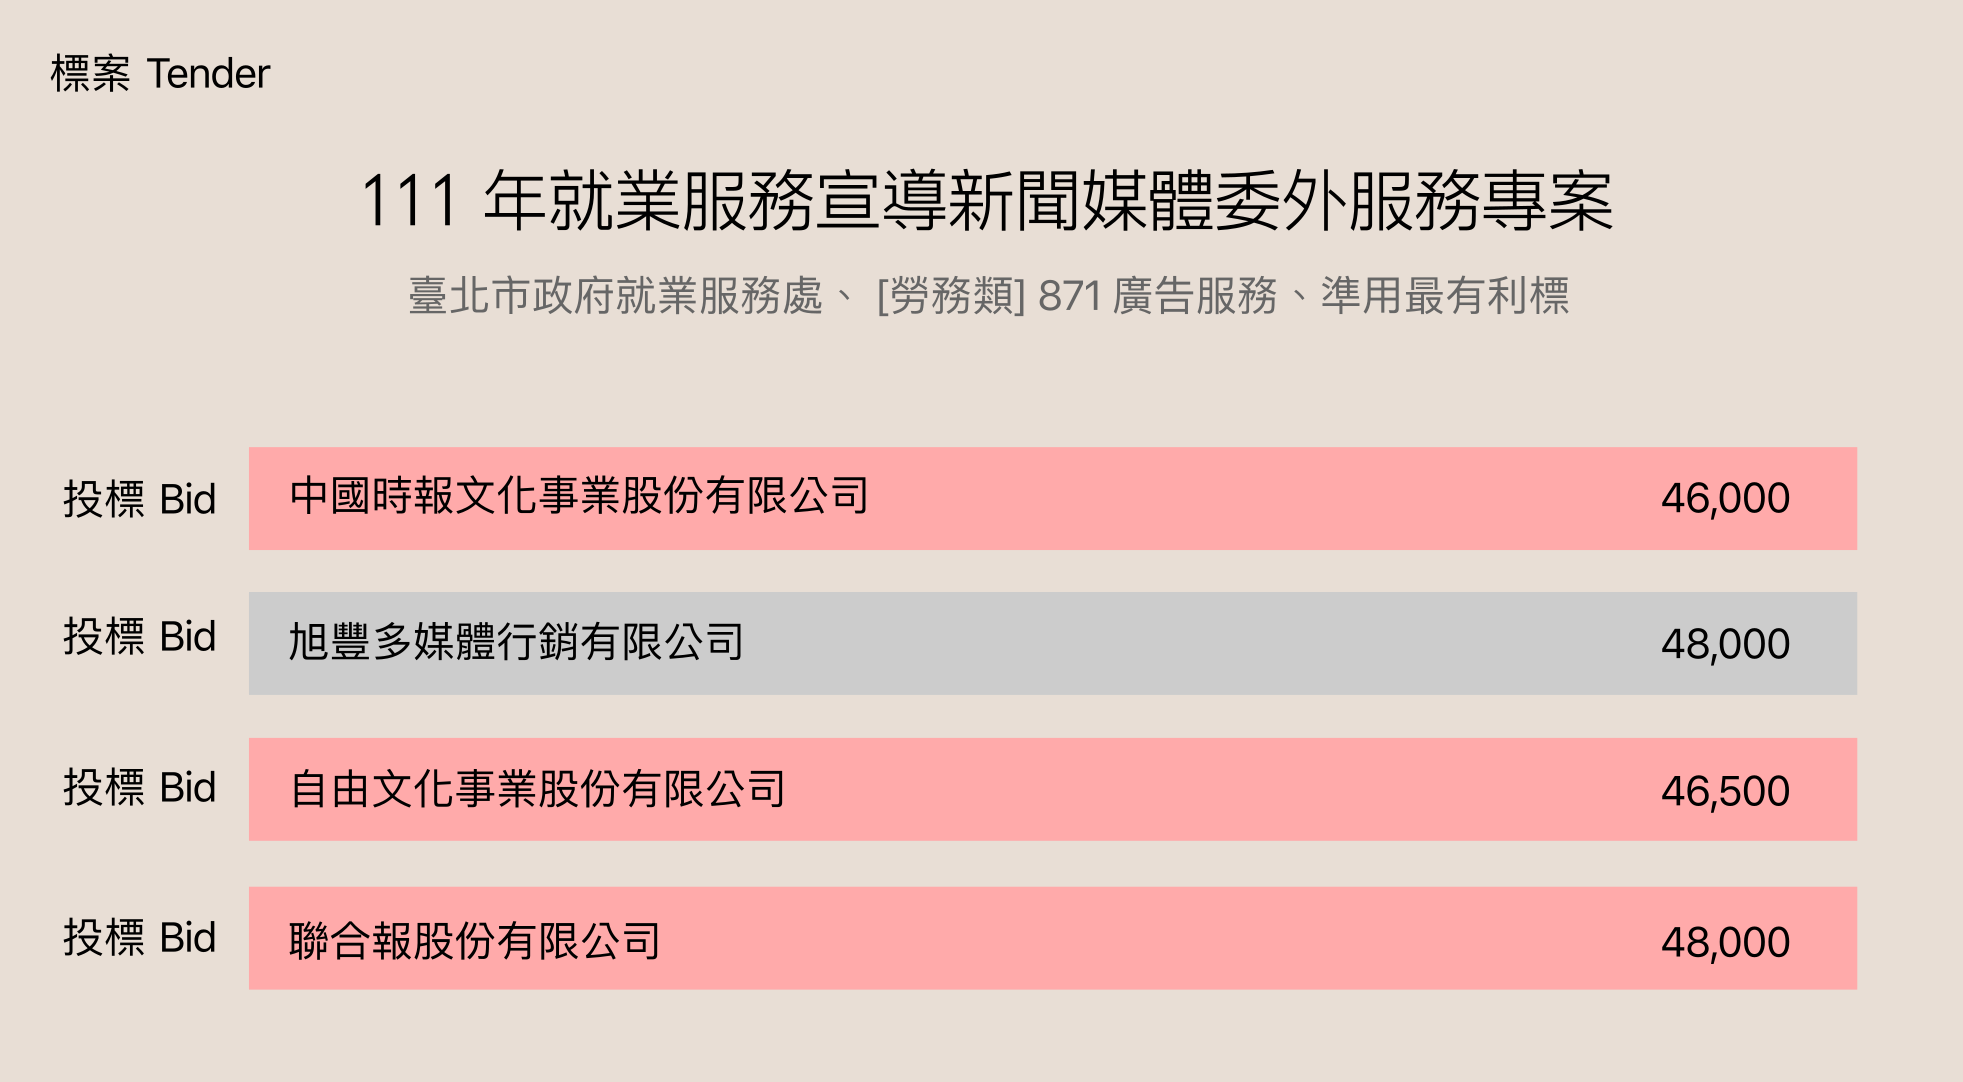
\includegraphics[width=0.95\textwidth,height=\textheight]{./graphs/tender-model.png}
\caption{Model of a Tender}
\end{figure}
\end{frame}

\begin{frame}
\begin{table}[!htbp] \centering \renewcommand*{\arraystretch}{1.1}\caption{Summary Statistics}\resizebox{\textwidth}{!}{
\begin{tabular}{lrrrrrrr}
\hline
\hline
Variable & N & Mean & Std. Dev. & Min & Pctl. 25 & Pctl. 75 & Max \\ 
\hline
ruling & 2412 &  &  &  &  &  &  \\ 
... DPP & 783 & 32.5\% &  &  &  &  &  \\ 
... INDEP & 272 & 11.3\% &  &  &  &  &  \\ 
... KMT & 1354 & 56.1\% &  &  &  &  &  \\ 
... 親民黨 & 3 & 0.1\% &  &  &  &  &  \\ 
competitors & 2412 & 3.322 & 2.764 & 1 & 1 & 4 & 28 \\ 
totalWinner & 2412 & 1.799 & 1.699 & 0 & 1 & 2 & 24 \\ 
valueAward & 2361 & 2944932.046 & 3791071.596 & 230 & 800080 & 3890000 & 60463000\\ 
\hline
\hline
\end{tabular}
}
\end{table}


\end{frame}

\hypertarget{empirical-findings}{%
\section{Empirical Findings}\label{empirical-findings}}

\begin{frame}{Upward Trend in Buying Ads}
\protect\hypertarget{upward-trend-in-buying-ads}{}
\begin{figure}
\centering
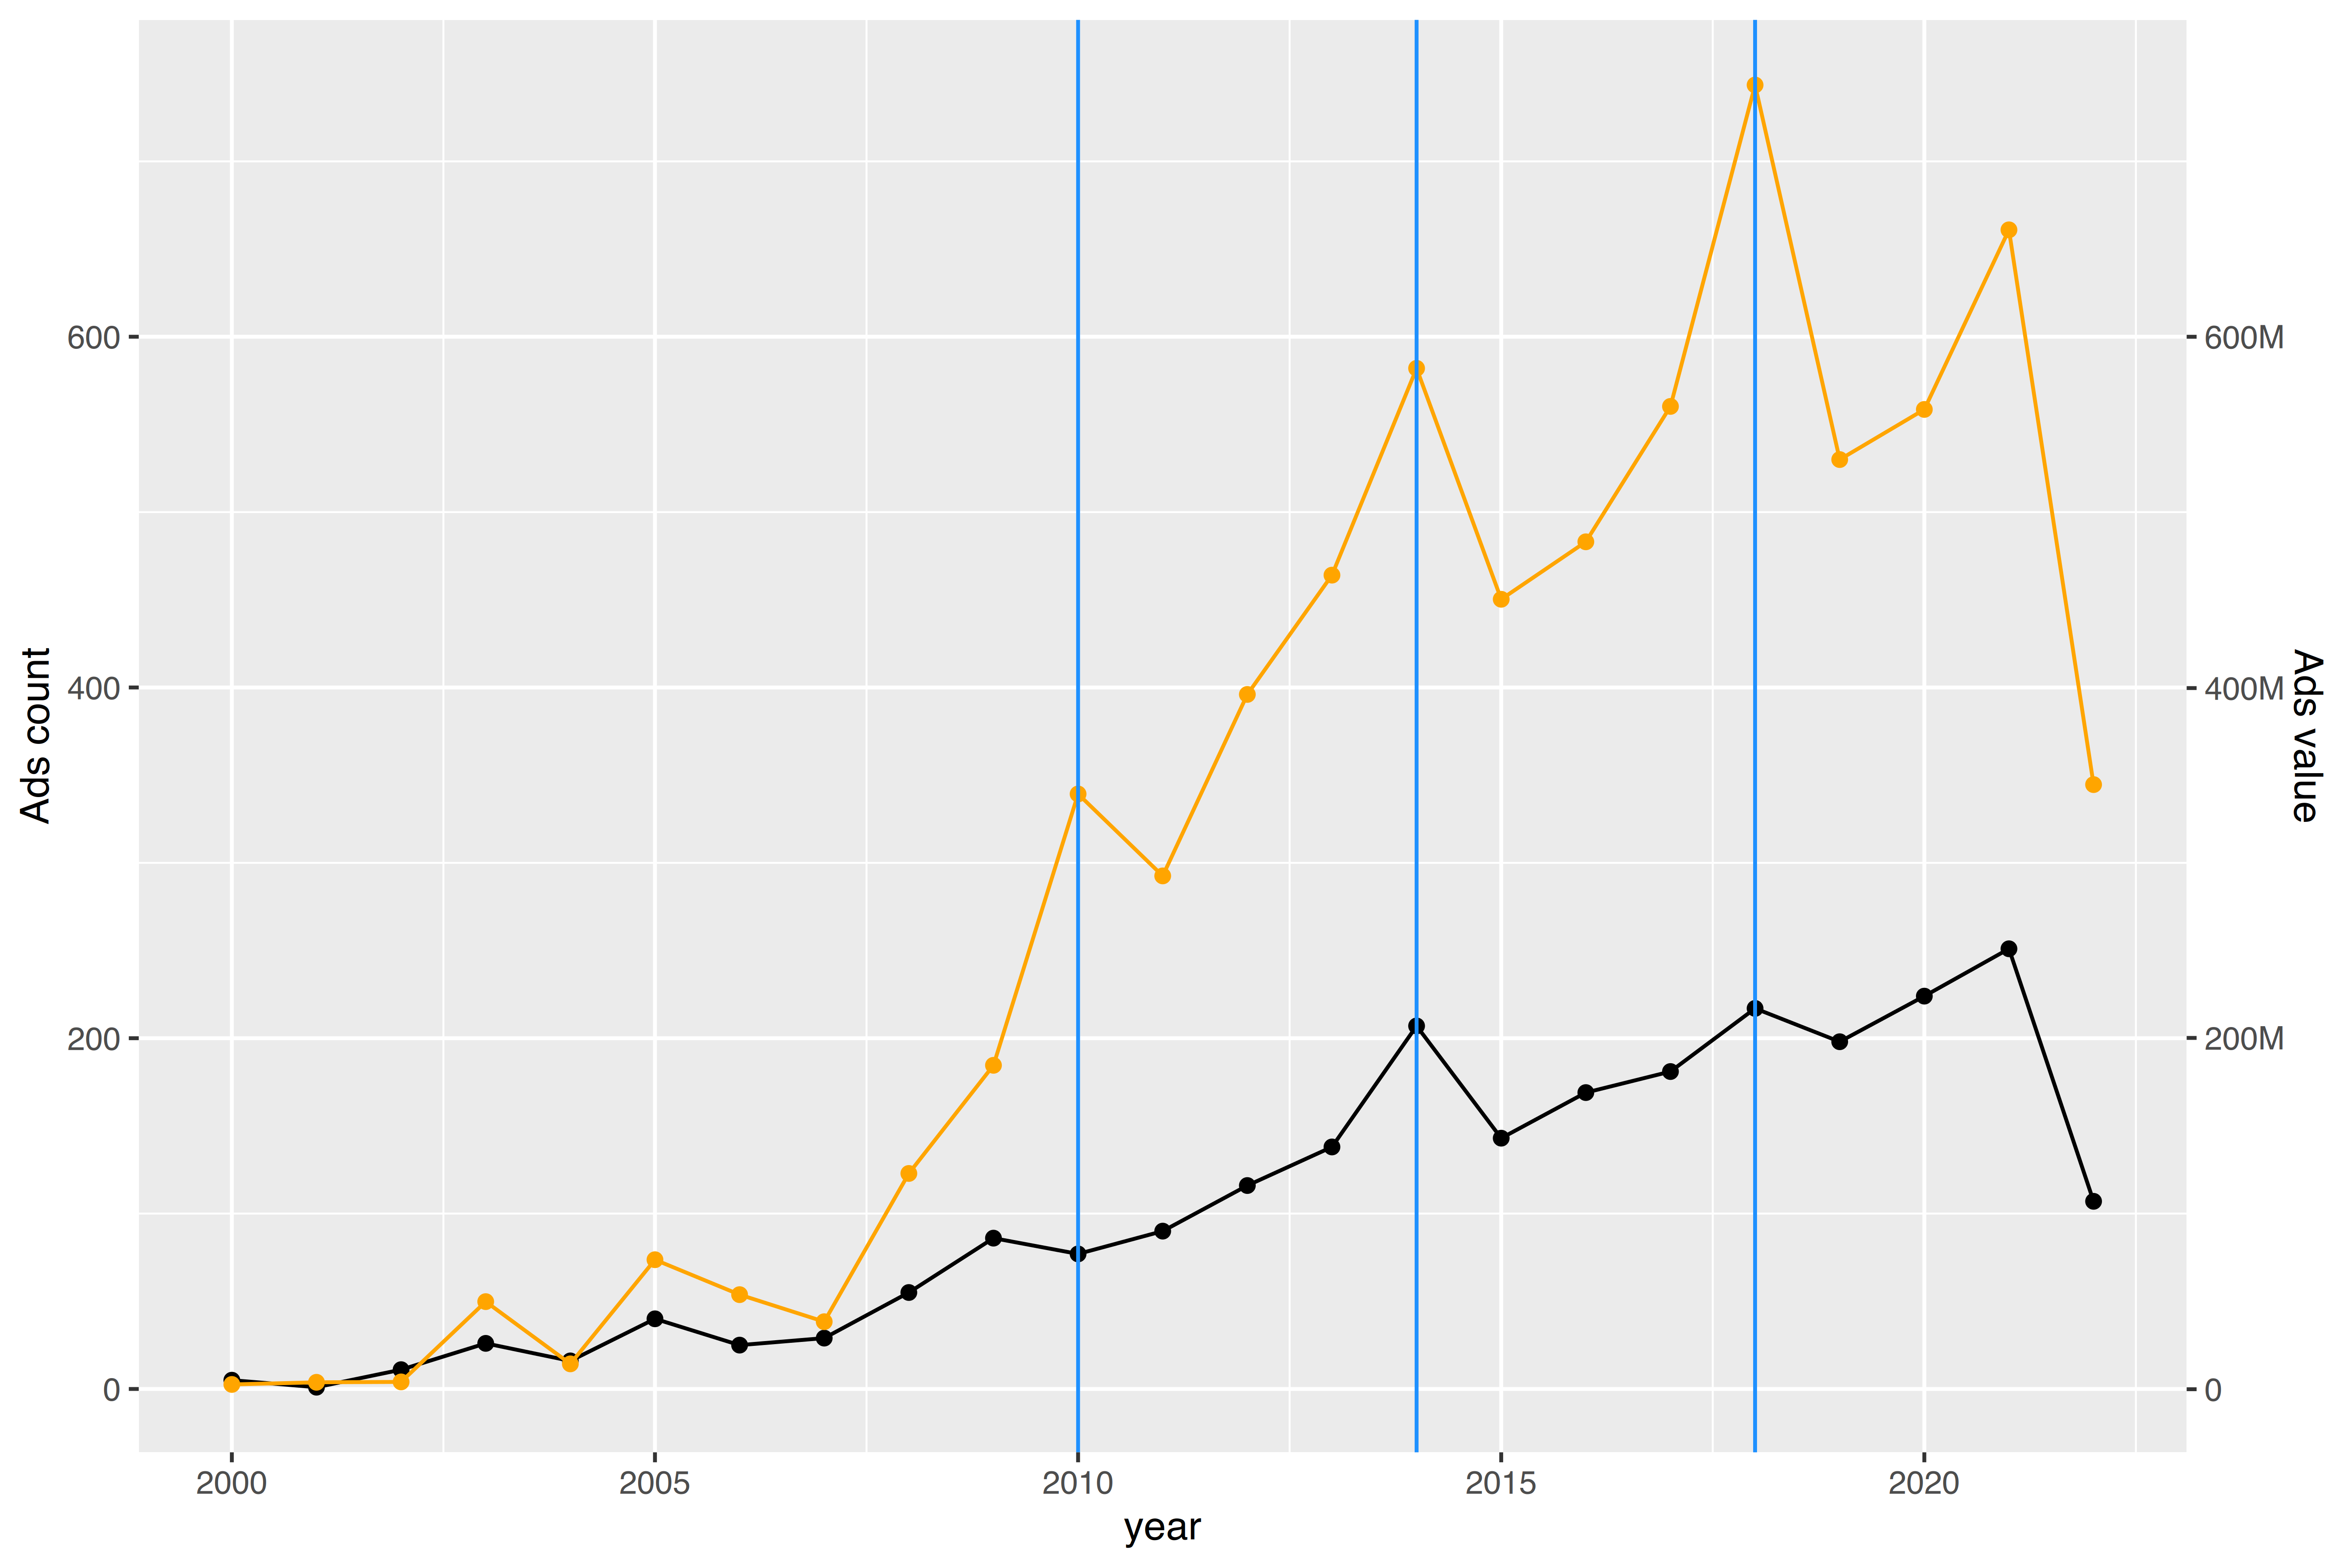
\includegraphics[width=0.75\textwidth,height=\textheight]{./graphs/tenderSummary-1.png}
\caption{Gov' Ads Quantity and Value by Year}
\end{figure}
\end{frame}

\begin{frame}
\begin{figure}
\centering
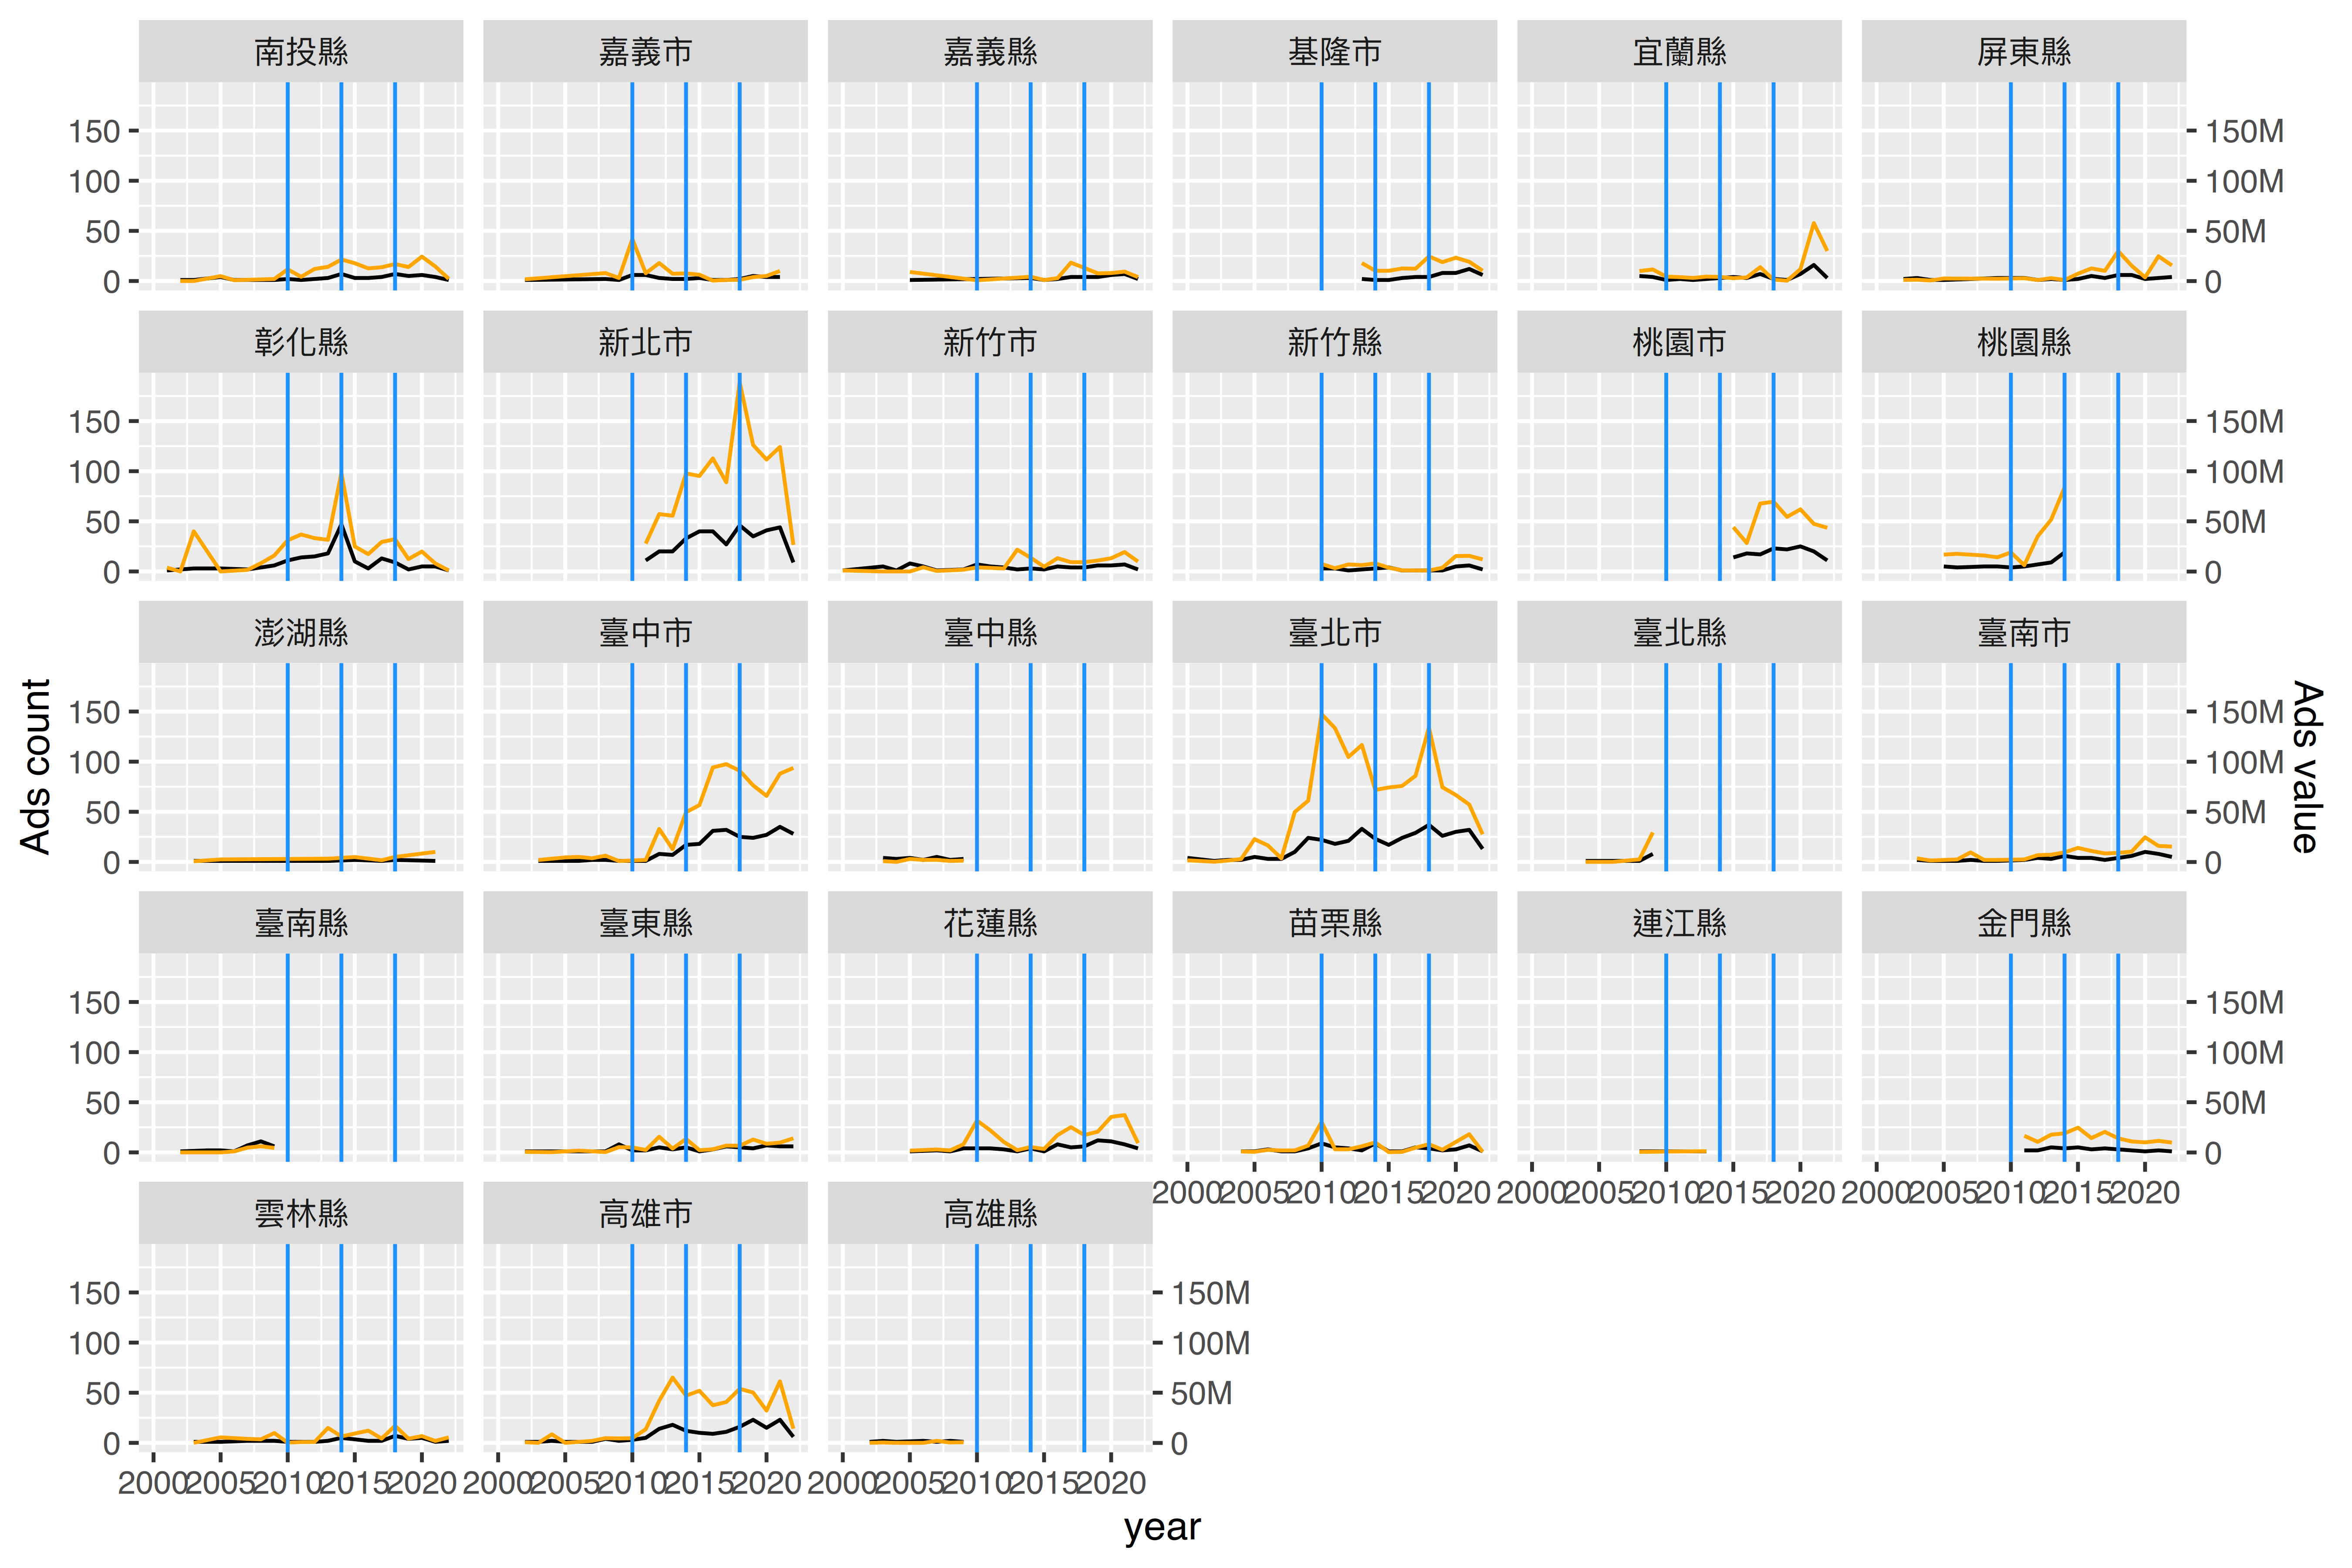
\includegraphics{./graphs/tenderSummary-2.png}
\caption{Gov' Ads Quantity and Value by County, Year}
\end{figure}
\end{frame}

\begin{frame}{Ads Buying in Election Years}
\protect\hypertarget{ads-buying-in-election-years}{}
\begin{figure}
\centering
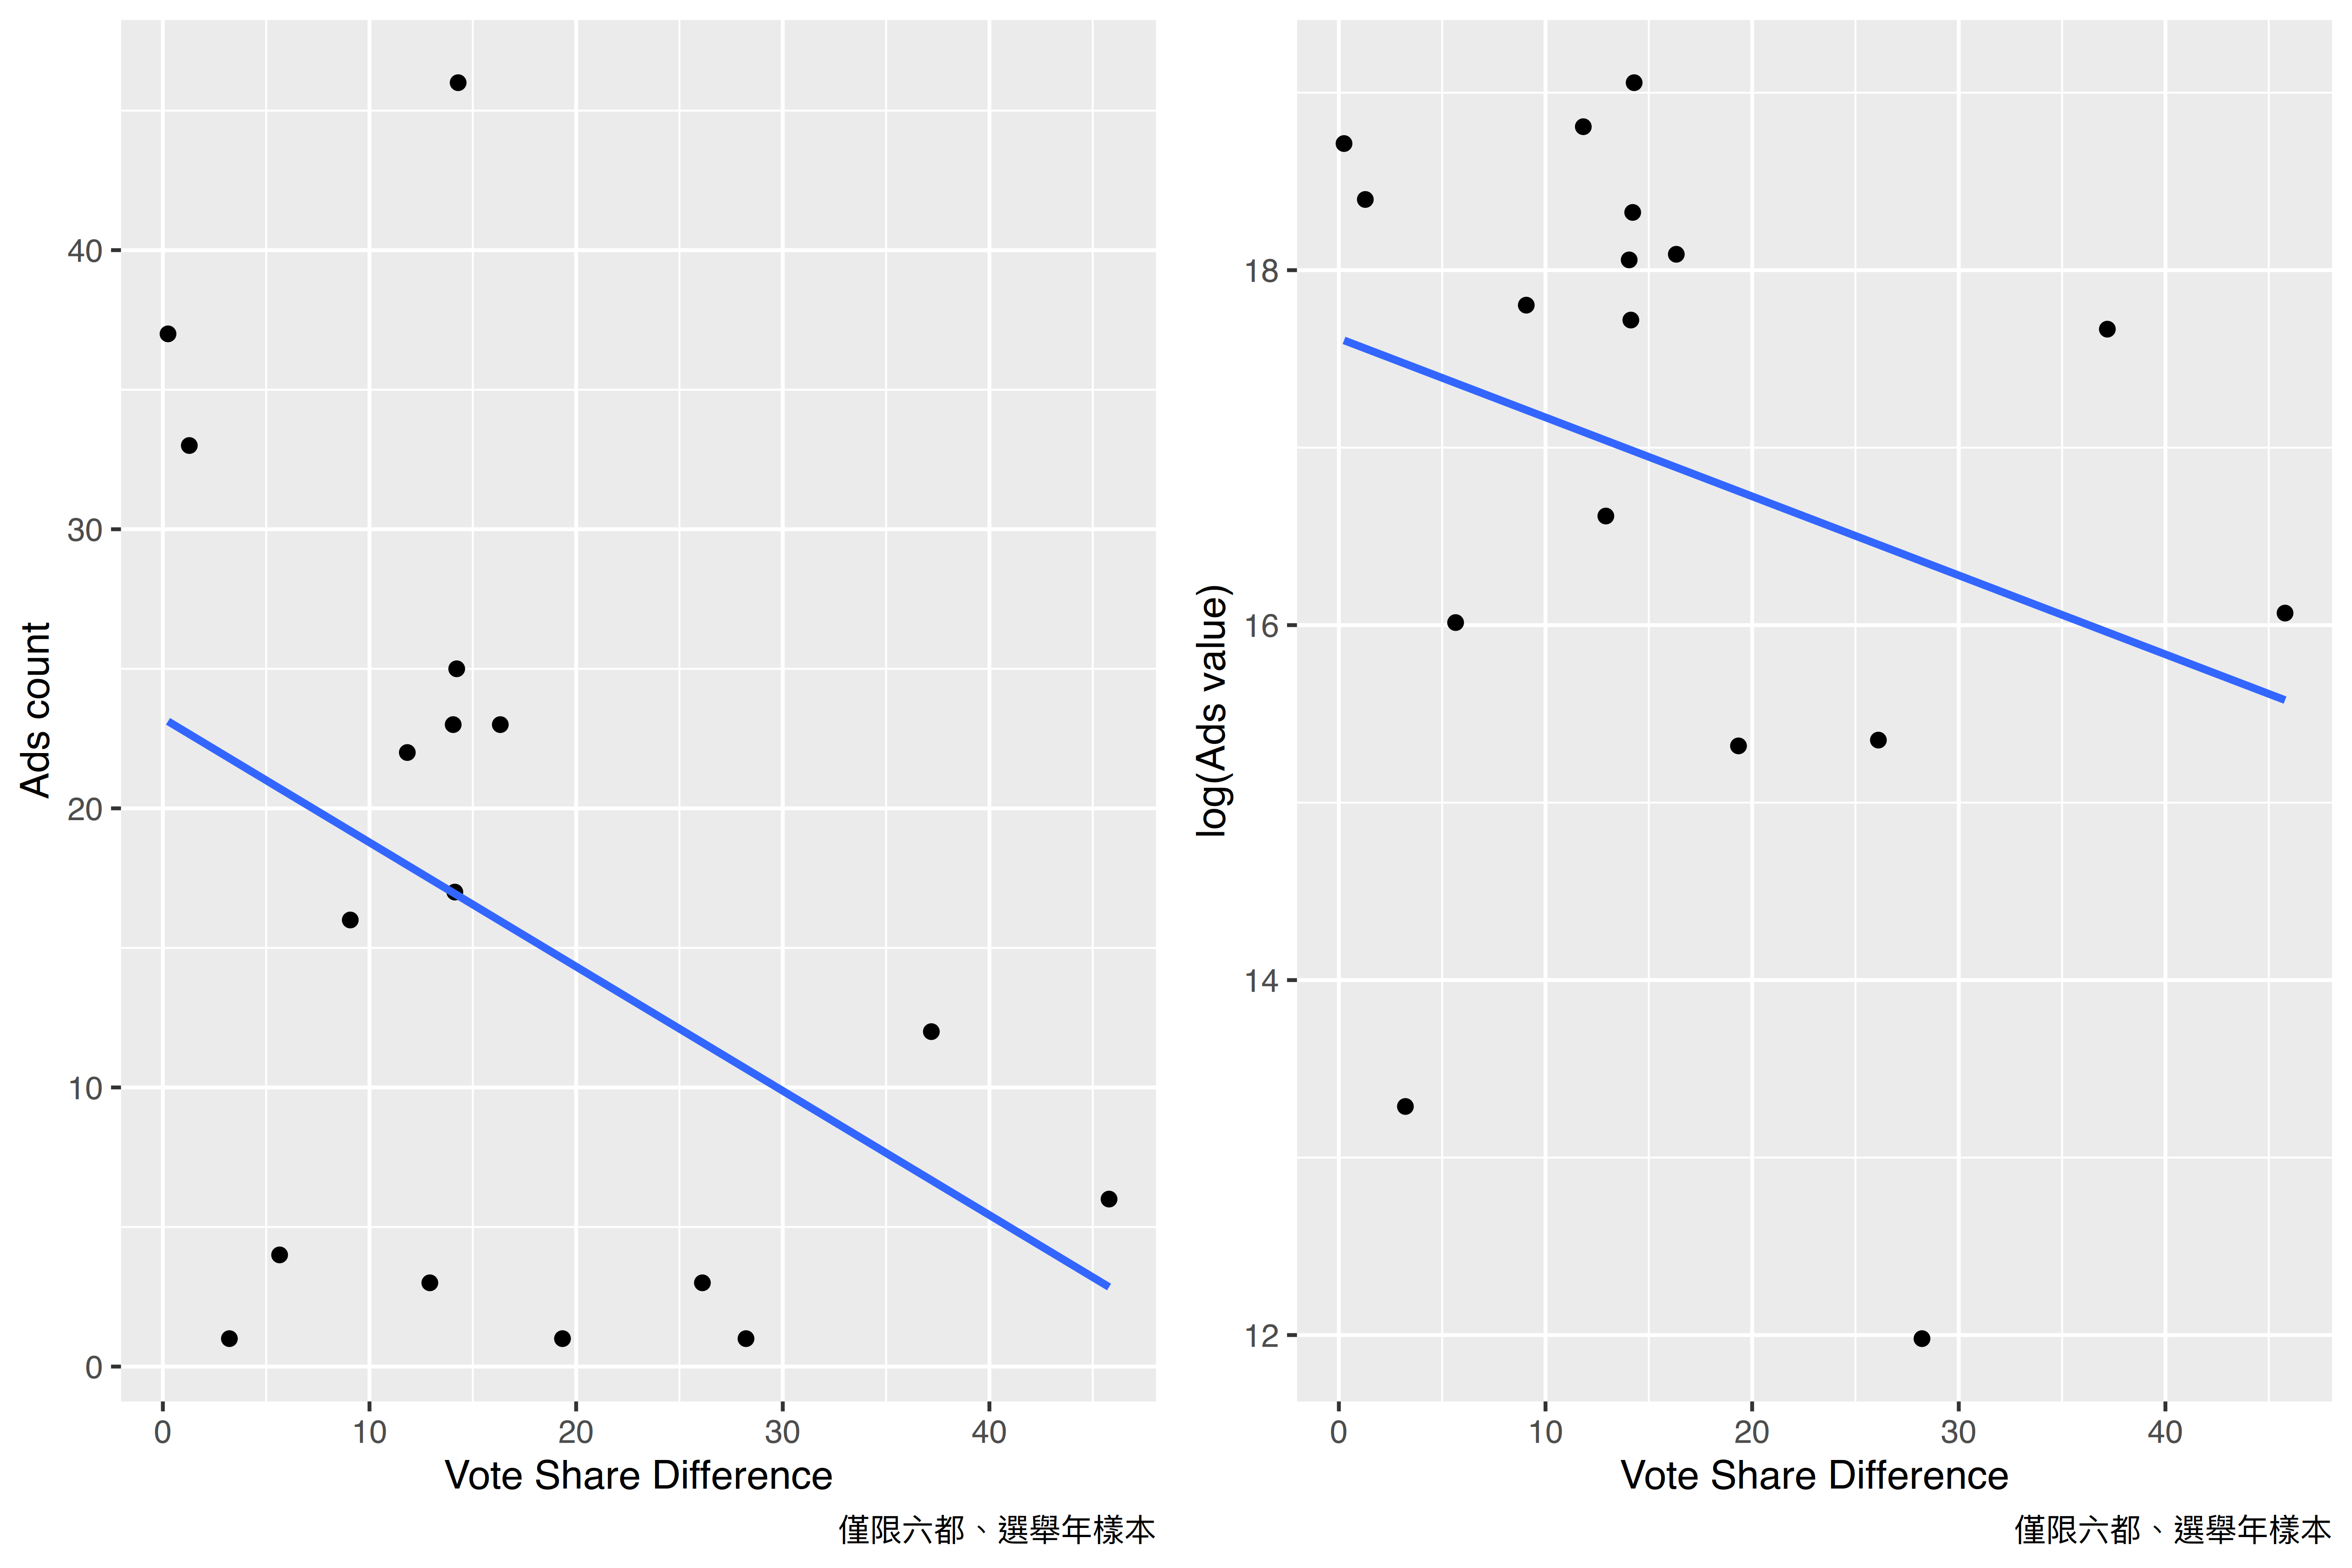
\includegraphics[width=0.75\textwidth,height=\textheight]{./graphs/electionTender-1.png}
\caption{Correlation Between Fierce Competition and Ads}
\end{figure}
\end{frame}

\begin{frame}{Partisan Preference on Ads Budget}
\protect\hypertarget{partisan-preference-on-ads-budget}{}
\begin{figure}
\centering
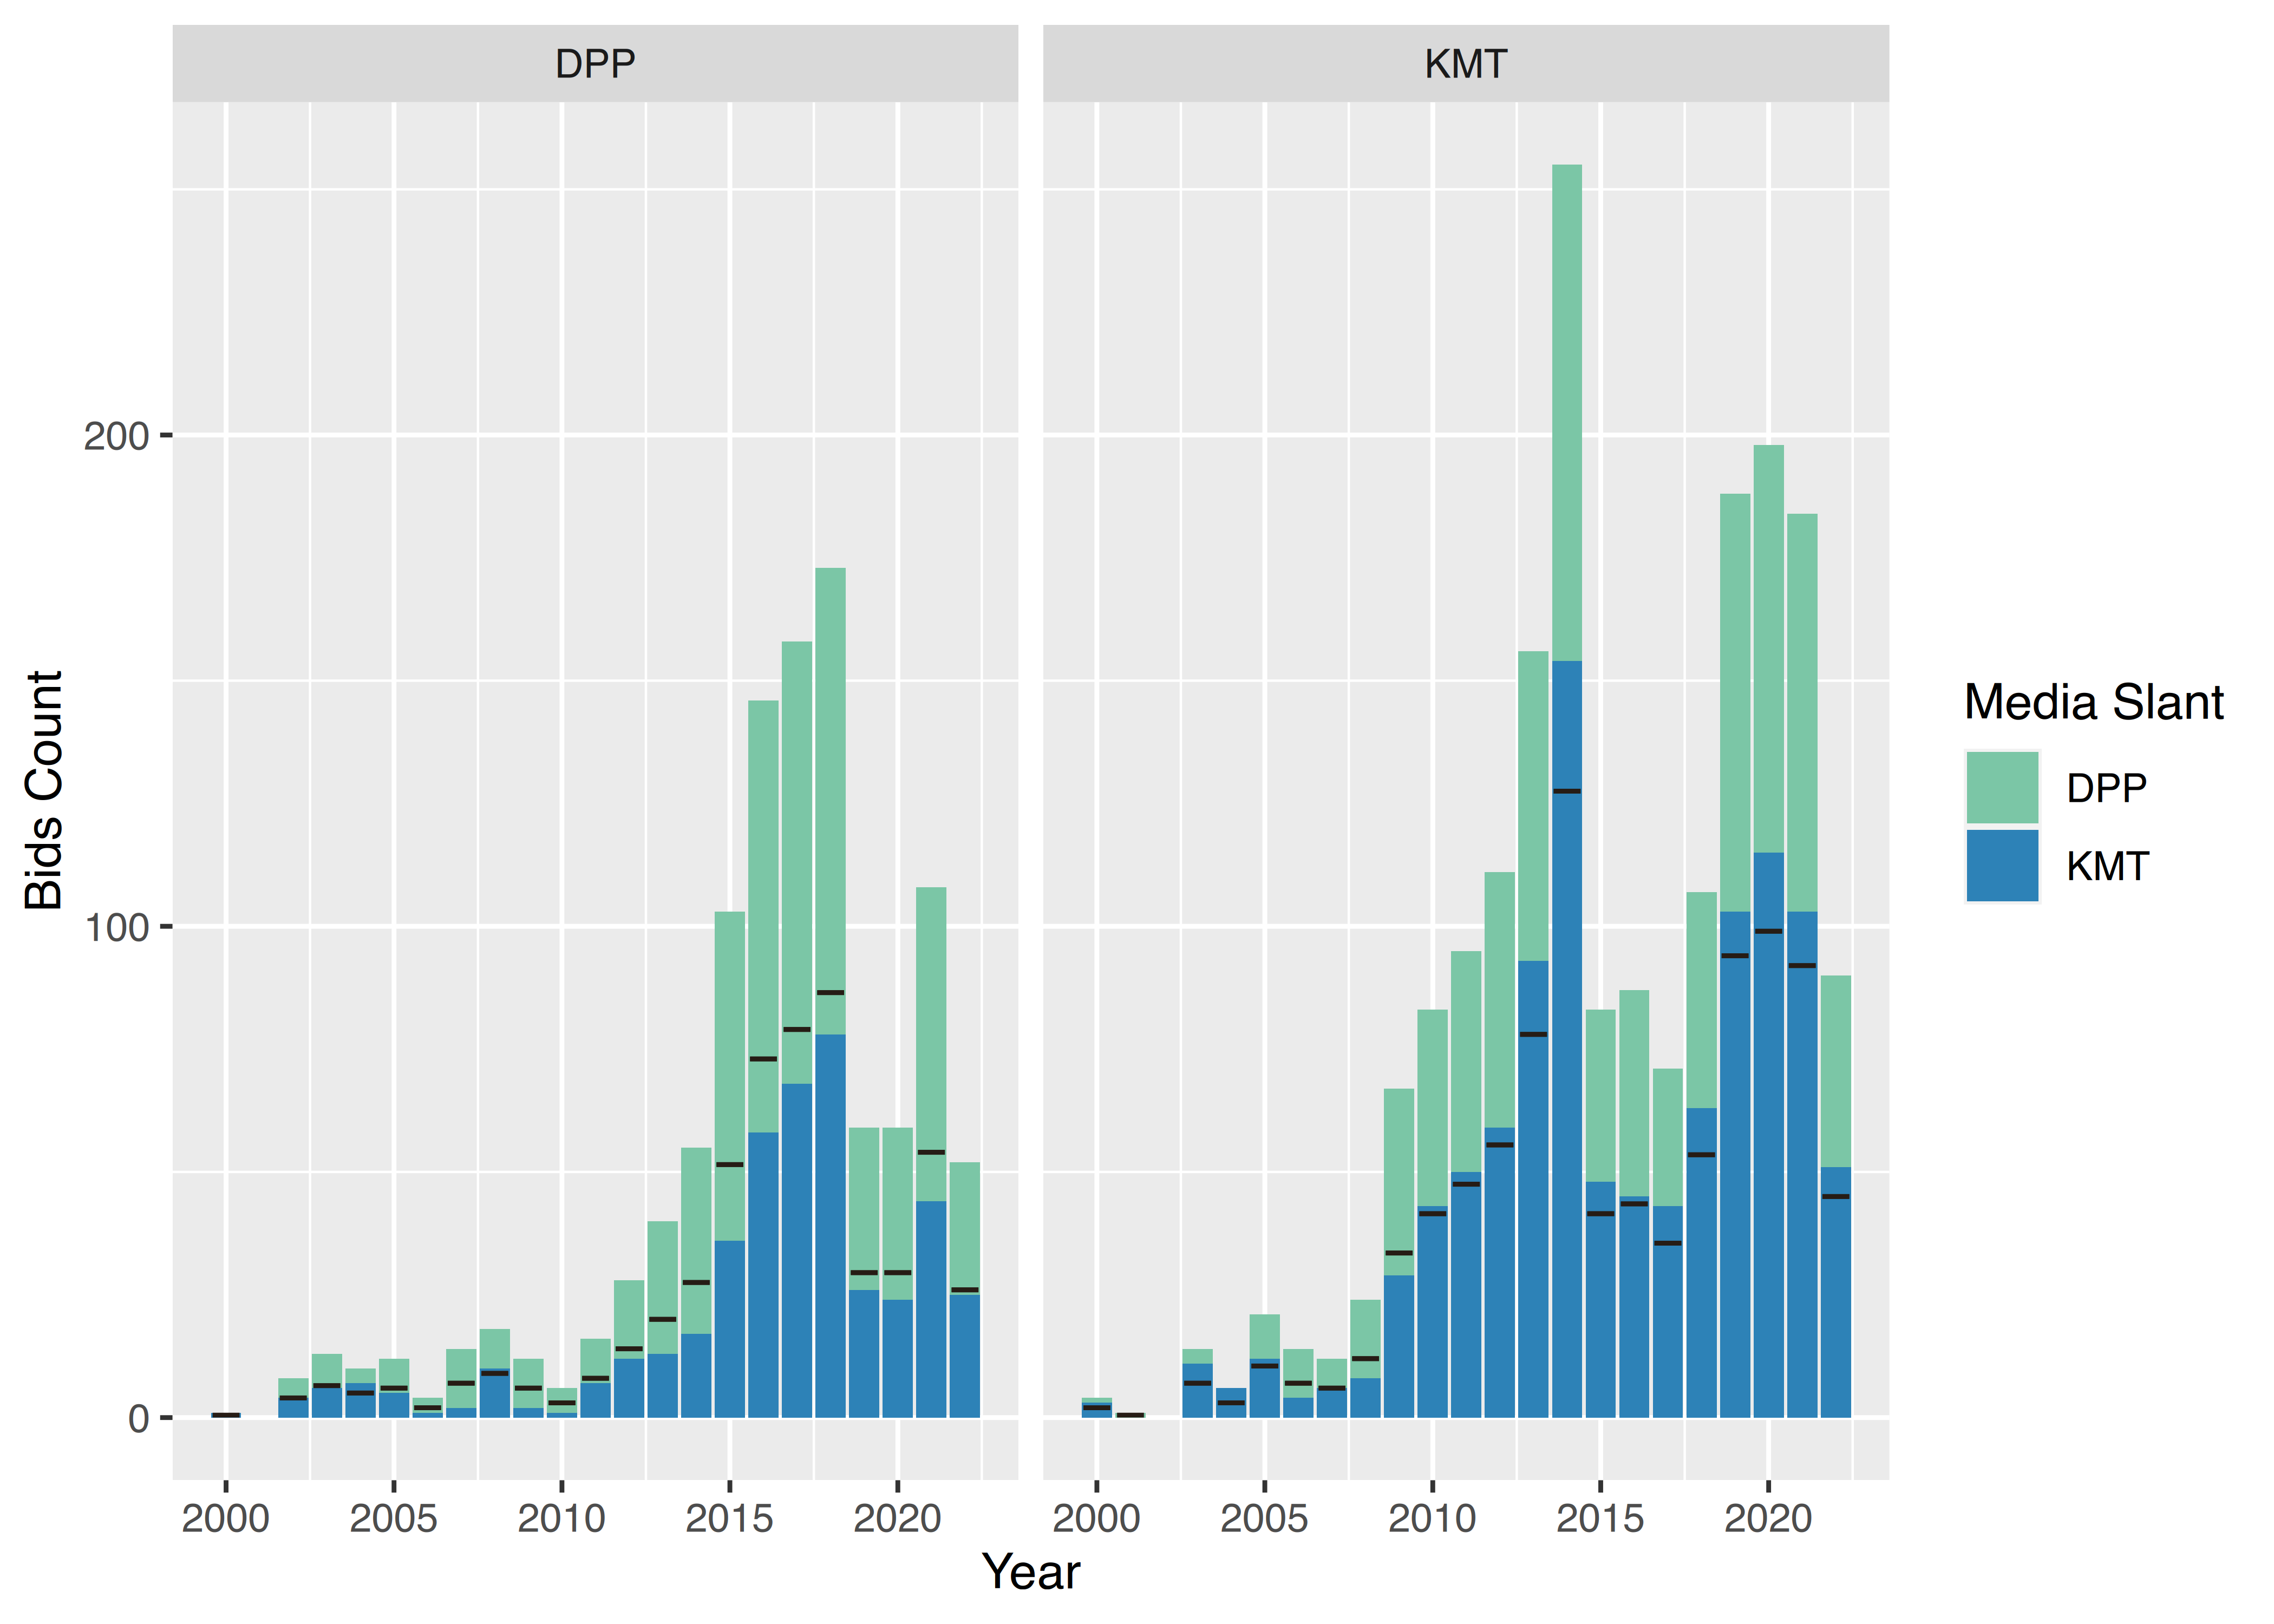
\includegraphics[width=0.7\textwidth,height=\textheight]{./graphs/partyBidPreference-1.png}
\caption{Number of Bids Won by Different Slant}
\end{figure}
\end{frame}

\begin{frame}
\begin{figure}
\centering
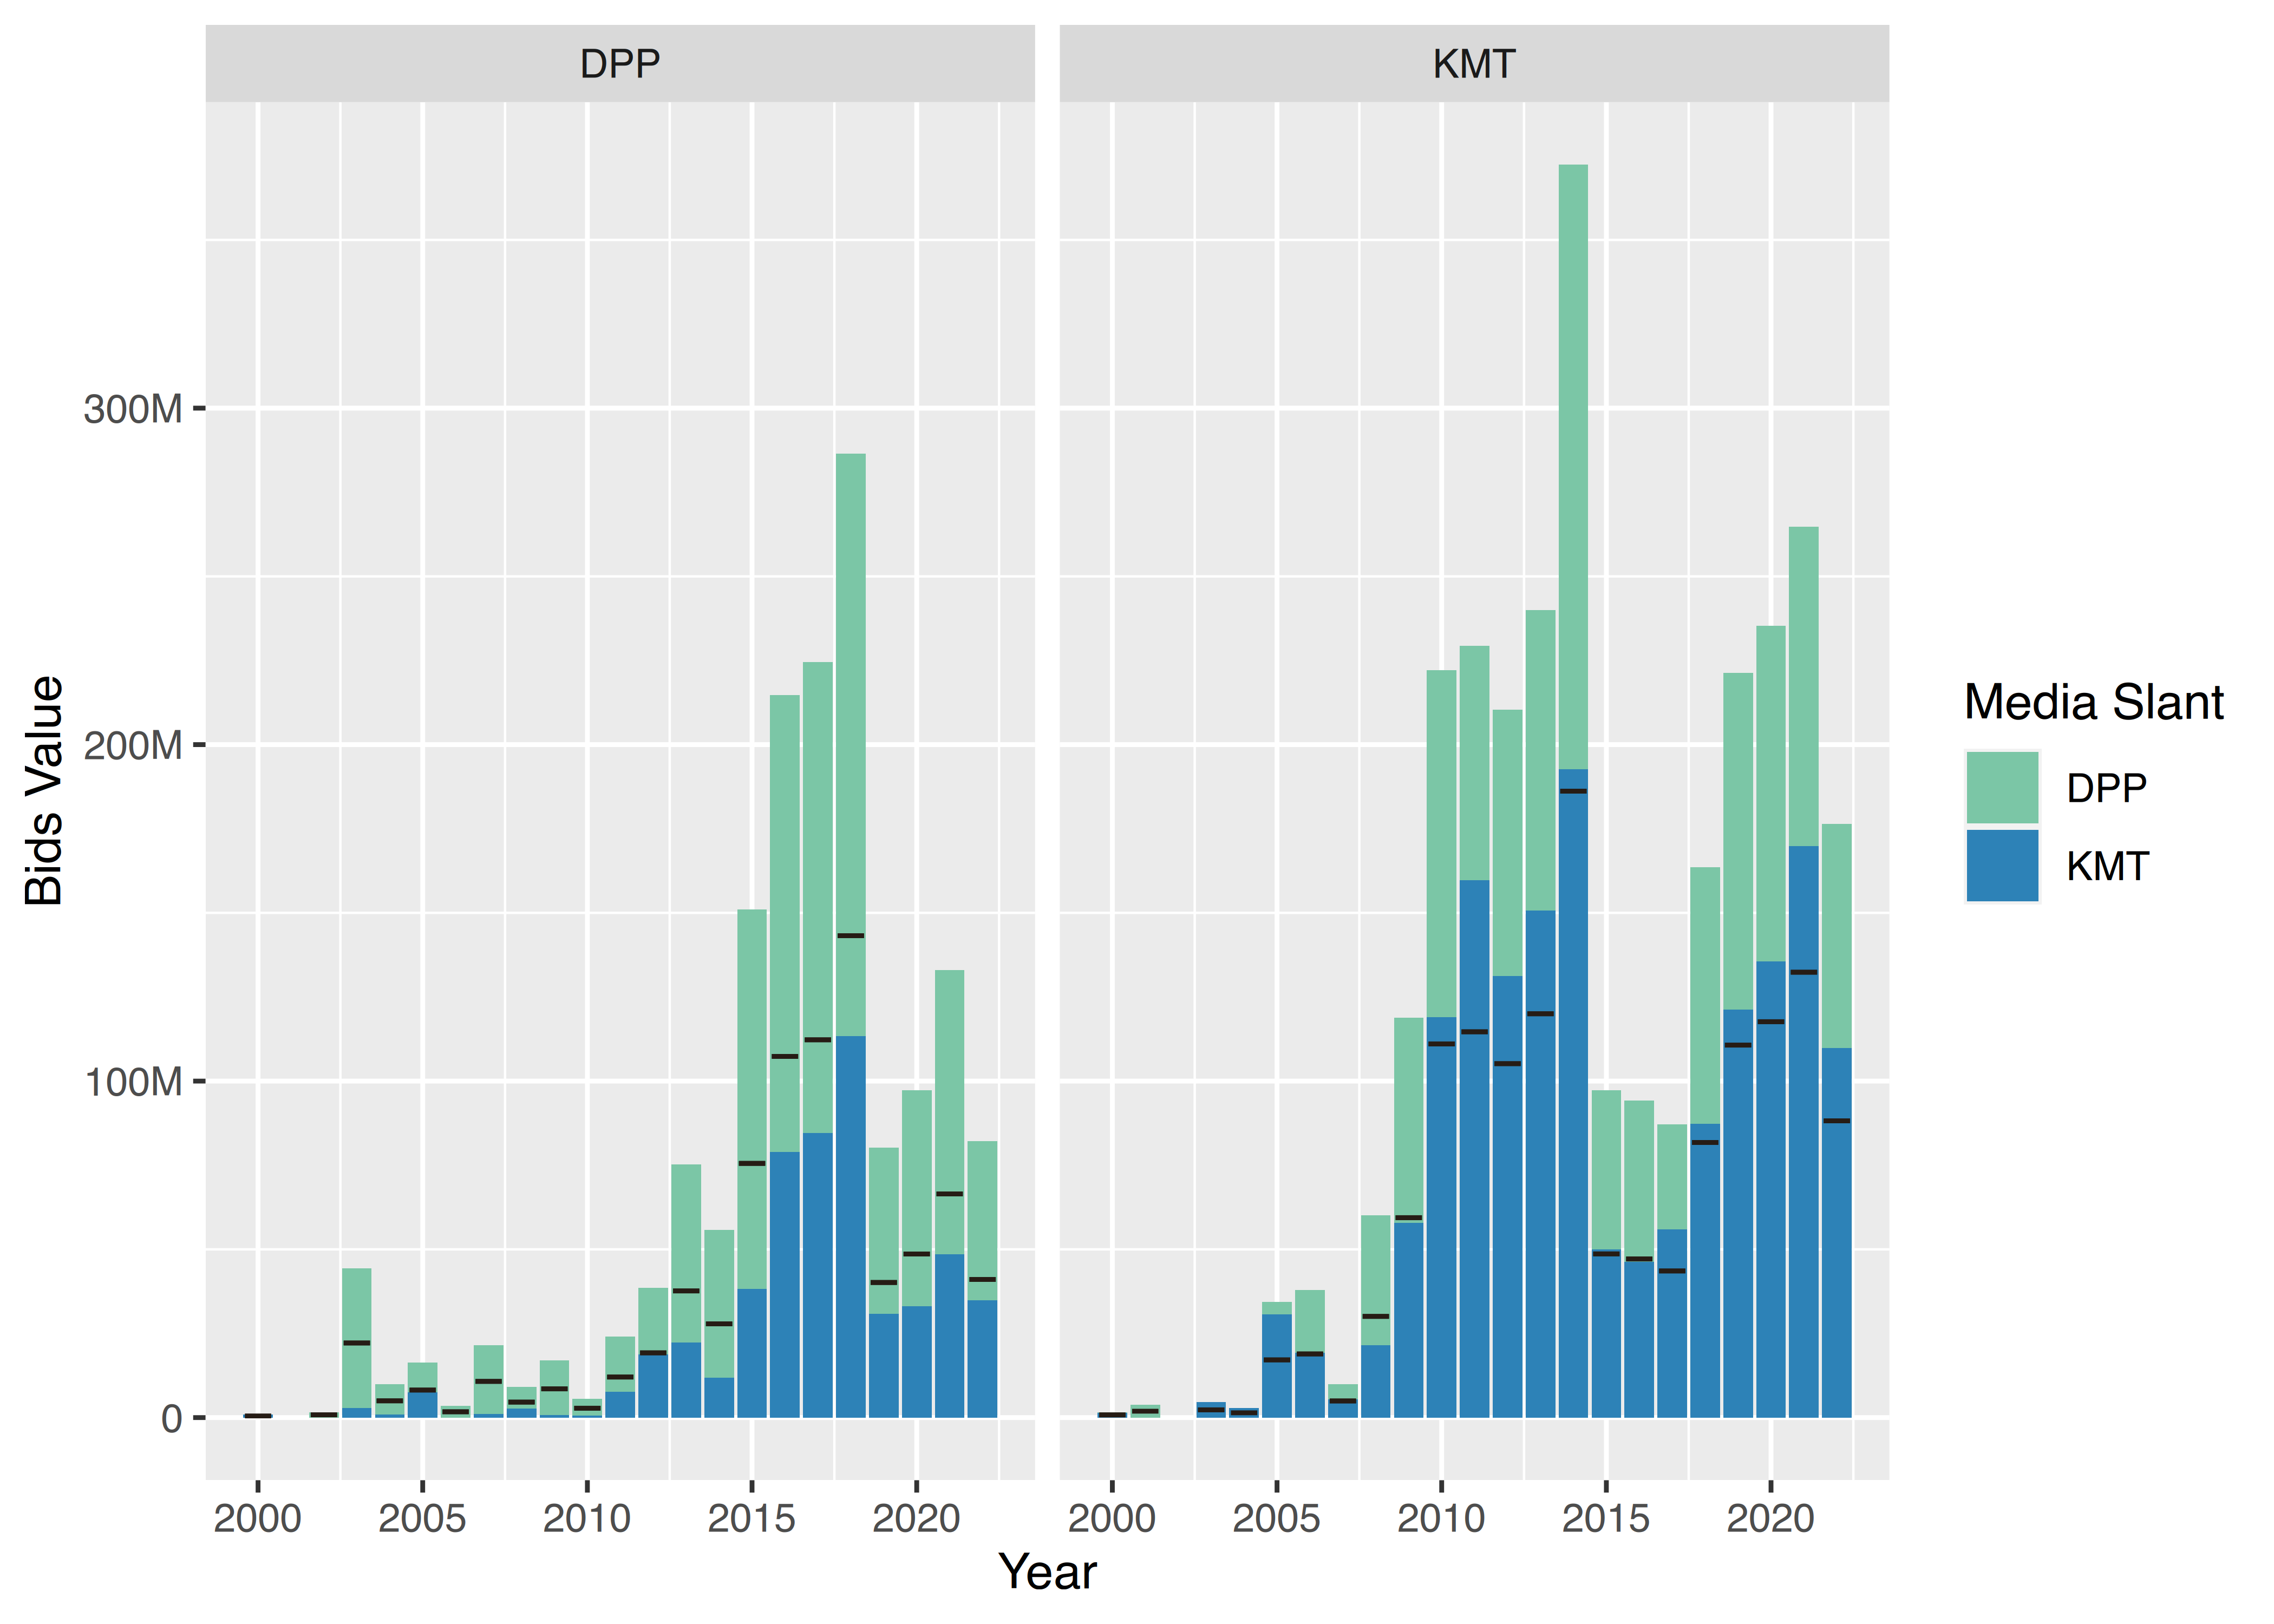
\includegraphics[width=0.9\textwidth,height=\textheight]{./graphs/partyBidPreference-2.png}
\caption{Value of Bids Won by Different Slant}
\end{figure}
\end{frame}

\begin{frame}{Governors' Preference on Aligned Media}
\protect\hypertarget{governors-preference-on-aligned-media}{}
\begin{columns}[T]
\begin{column}{0.6\textwidth}
\begin{block}{Sample:}
\protect\hypertarget{sample}{}
\textbf{Bids} to tenders that were\ldots{}

\begin{itemize}
\tightlist
\item
  opened by KMT/DPP local governments.
\item
  involved by both pan-blue/green media

  \begin{itemize}
  \tightlist
  \item
    旺中、聯合、TVBS、自由、三立、民視
  \end{itemize}
\item
  governed by ``Most Advantageous 最有利標'' rule
\end{itemize}
\end{block}
\end{column}

\begin{column}{0.3\textwidth}
\begin{block}{Outcome}
\protect\hypertarget{outcome}{}
\begin{itemize}
\tightlist
\item
  Winning or not
\item
  \(\ln(\text{Value of the bid})\)
\end{itemize}
\end{block}
\end{column}
\end{columns}

\begin{block}{OLS Specification}
\protect\hypertarget{ols-specification}{}
\[
Y_{itcm} = \beta_0 + \beta_1 \text{Alignment}_{tcm} \times \text{Ruling}_{tc} + X_i + \delta_t + \delta_c
\]

for bid \(i\), year \(t\), opened by county \(c\), and issued by media
conglomerate \(m\)
\end{block}
\end{frame}

\begin{frame}
\begin{table}[!htbp] \centering \renewcommand*{\arraystretch}{1.1}\caption{Summary Statistics on Regression Sample}\resizebox{0.8\textwidth}{!}{
        \begin{tabular}{lrrrrrrr}
            \hline
            \hline
            Variable    & N    & Mean        & Std. Dev.   & Min    & Pctl. 25 & Pctl. 75 & Max      \\
            \hline
            ruling      & 1256 &             &             &        &          &          &          \\
            ... DPP     & 489  & 38.9\%      &             &        &          &          &          \\
            ... KMT     & 767  & 61.1\%      &             &        &          &          &          \\
            slant       & 1256 &             &             &        &          &          &          \\
            ... DPP     & 479  & 38.1\%      &             &        &          &          &          \\
            ... KMT     & 777  & 61.9\%      &             &        &          &          &          \\
            winner      & 1256 &             &             &        &          &          &          \\
            ... No      & 320  & 25.5\%      &             &        &          &          &          \\
            ... Yes     & 936  & 74.5\%      &             &        &          &          &          \\
            competitors & 1256 & 6.649       & 2.376       & 2      & 5        & 8        & 26       \\
            totalWinner & 1256 & 4.438       & 2.354       & 1      & 3        & 6        & 10       \\
            valueAward  & 1256 & 5573532.826 & 3357681.298 & 295000 & 3e+06    & 7700000  & 23999300 \\
            \hline
            \hline
        \end{tabular}
    }
\end{table}


\end{frame}

\begin{frame}
\begin{table}
  \caption{Regression: Winning}
  \centering
  \resizebox{0.9\textwidth}{!}{
    \begin{tabular}[t]{lccccc}
      \toprule
                                            & Full            & Full (FEs)      & Full (by Ruling Pty) & Post-2011       & Post-2016       \\
      \midrule
      alignment                             & \num{0.093}***  & \num{0.092}***  & \num{0.150}***       & \num{0.149}***  & \num{0.182}***  \\
                                            & (\num{0.022})   & (\num{0.023})   & (\num{0.037})        & (\num{0.038})   & (\num{0.044})   \\
      alignment \(\times\) ruling=KMT       &                 &                 & \num{-0.096}*        & \num{-0.075}    & \num{-0.140}*   \\
                                            &                 &                 & (\num{0.047})        & (\num{0.048})   & (\num{0.059})   \\
      competitors                           & \num{-0.059}*** & \num{-0.055}*** & \num{-0.055}***      & \num{-0.054}*** & \num{-0.047}*** \\
                                            & (\num{0.006})   & (\num{0.007})   & (\num{0.007})        & (\num{0.007})   & (\num{0.008})   \\
      totalWinner                           & \num{0.115}***  & \num{0.111}***  & \num{0.110}***       & \num{0.108}***  & \num{0.096}***  \\
                                            & (\num{0.005})   & (\num{0.005})   & (\num{0.005})        & (\num{0.005})   & (\num{0.007})   \\
      \midrule
      Num.Obs.                              & \num{1256}      & \num{1256}      & \num{1256}           & \num{1179}      & \num{758}       \\
      R2 Adj.                               & \num{0.310}     & \num{0.307}     & \num{0.309}          & \num{0.312}     & \num{0.278}     \\
      Std.Errors                            & by: filename    & by: filename    & by: filename         & by: filename    & by: filename    \\
      FE: county                            &                 & X               & X                    & X               & X               \\
      FE: year                              &                 & X               & X                    & X               & X               \\
      p-value: Alignment \(\times\) KMT = 0 & NA              & NA              & \num{0.0657}         & \num{0.0262}    & \num{0.3553}    \\
      \bottomrule
      \multicolumn{6}{l}{\rule{0pt}{1em}+ p $<$ 0.1, * p $<$ 0.05, ** p $<$ 0.01, *** p $<$ 0.001}                                         \\
    \end{tabular}
  }
\end{table}

\end{frame}

\begin{frame}
\begin{table}
  \caption{Regression: Bid Value}
  \centering
  \resizebox{0.9\textwidth}{!}{
    \begin{tabular}[t]{lccccc}
      \toprule
                                            & Full            & Full (FEs)      & Full (by Ruling Pty) & Post-2011       & Post-2016       \\
      \midrule
      alignment                             & \num{0.021}     & \num{0.029}     & \num{0.199}***       & \num{0.181}***  & \num{0.174}**   \\
                                            & (\num{0.032})   & (\num{0.031})   & (\num{0.051})        & (\num{0.049})   & (\num{0.057})   \\
      alignment \(\times\) ruling=KMT       &                 &                 & \num{-0.278}***      & \num{-0.259}*** & \num{-0.165}*   \\
                                            &                 &                 & (\num{0.063})        & (\num{0.061})   & (\num{0.072})   \\
      competitors                           & \num{0.061}***  & \num{0.050}***  & \num{0.051}***       & \num{0.045}**   & \num{0.008}     \\
                                            & (\num{0.013})   & (\num{0.014})   & (\num{0.014})        & (\num{0.014})   & (\num{0.015})   \\
      totalWinner                           & \num{-0.161}*** & \num{-0.155}*** & \num{-0.156}***      & \num{-0.151}*** & \num{-0.118}*** \\
                                            & (\num{0.014})   & (\num{0.015})   & (\num{0.015})        & (\num{0.015})   & (\num{0.016})   \\
      \midrule
      Num.Obs.                              & \num{1572}      & \num{1572}      & \num{1572}           & \num{1433}      & \num{915}       \\
      R2 Adj.                               & \num{0.154}     & \num{0.238}     & \num{0.244}          & \num{0.261}     & \num{0.261}     \\
      Std.Errors                            & by: filename    & by: filename    & by: filename         & by: filename    & by: filename    \\
      FE: county                            &                 & X               & X                    & X               & X               \\
      FE: year                              &                 & X               & X                    & X               & X               \\
      p-value: Alignment \(\times\) KMT = 0 & NA              & NA              & \num{0.206}          & \num{0.1934}    & \num{0.7816}    \\
      \bottomrule
      \multicolumn{6}{l}{\rule{0pt}{1em}+ p $<$ 0.1, * p $<$ 0.05, ** p $<$ 0.01, *** p $<$ 0.001}                                         \\
    \end{tabular}
  }
\end{table}

\end{frame}

\hypertarget{conclusions}{%
\section{Conclusions}\label{conclusions}}

\begin{frame}{Conclusions}
\begin{itemize}
\tightlist
\item
  Increased ads spending in election year, suggesting incumbency
  advantage.
\item
  Both KMT and DPP have preference toward aligned media

  \begin{itemize}
  \tightlist
  \item
    while KMT prefers equalizing the value of tenders, DPP prefers
    giving pro-green media valuable cases
  \end{itemize}
\item
  Potential impact of decreased commercial ads on media capture
\item
  Limits of the findings:

  \begin{itemize}
  \tightlist
  \item
    Lack of exogenous instrument to identify causal effect
  \item
    Media's \emph{capability} unobserved
  \item
    Differed public opinion might change government's preference on
    buying ads
  \end{itemize}
\end{itemize}
\end{frame}

\end{document}
